\documentclass{article} % For LaTeX2e
\usepackage{nips15submit_e,times}
\usepackage{hyperref}
\usepackage{url}
\usepackage{graphicx}
\usepackage{subcaption}
\usepackage{amsthm}

\theoremstyle{definition}
\newtheorem{definition}{Definition}[section]
\newtheorem{theorem}{Theorem}[section]
\newtheorem{corollary}{Corollary}[theorem]
\newtheorem{lemma}[theorem]{Lemma}

%\documentstyle[nips14submit_09,times,art10]{article} % For LaTeX 2.09
\title{}
\author{}
\newcommand{\fix}{\marginpar{FIX}}
\newcommand{\new}{\marginpar{NEW}}
\nipsfinalcopy % Uncomment for camera-ready version
\begin{document}

\maketitle

\begin{abstract}

\end{abstract}

\section{Basics}

\begin{definition}[Markov Property]
A stochastic process has the Markov property if the conditional
probability distribution of future states of the process (conditional
on both past and present states) depends only upon the present state,
not on the sequence of events that preceded it.
\[
P(x_{n+1} | x_{n}, x_{n-1}, \dots, x_{1}) = P(x_{n+1} | x_{n})
\]
\end{definition}

\begin{definition}[k-order Markov Chain]
A Markov chain of order $k$ has the property that:
\[
P(x_{n+1} | x_{n}, x_{n-1}, \dots, x_{1}) = P(x_{n+1} | x_{n}, \dots, x_{n-(k-1)})
\]
The future state $x_{n+1}$ depends on the past $k$ states. Remembering
$k$ states restores the Markov property and a larger memory grants no
further predictive power.
\end{definition}

\section{Partial Observability}
In the context of reinforcement learning, partial observability is a
term used to describe environments in which an agent's perceptions do
not provide complete information about the true state of the
environment. This problem is also known as \textit{incomplete
  perception}, \textit{perceptual aliasing}, or simply \textit{hidden
  state}.

One cause of partial observability is sensor noise, in which two
different states appear to be the same state due to noise in
observations. Another cause is perceptual aliasing, in which multiple
environment states are indistinguishable given the
observations. Figure \ref{fig:functions} illustrates these cases.


\begin{definition}[Observability]
Assuming access to the true state distribution $S$ of an environment
as well as the observation distribution $O$, the observability
$\mathcal{O}$ of the environment is given by conditional entropy of
the true states given the observations, divided by the entropy of the
states.
\[
\mathcal{O} = 1 - \frac{H(S|O)}{H(S)}
\]
The observability quantifies how much information the observations
possess about the true environment state. Observability is always
between zero and one: an observability of zero indicates the
observations are no help in understanding the environment's state. An
observability of one implies the observations fully determine the true
state. Observability measure the degree of bijectivity in an
environment's mapping from states to observations.
\end{definition}

\begin{figure}
\centering
\begin{subfigure}{.3\textwidth}
  \centering
  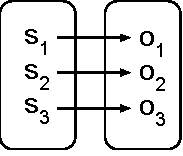
\includegraphics[width=.6\linewidth]{figures/bijection}
  \caption{Fully Observed}
  \label{fig:bijection}
\end{subfigure}
\begin{subfigure}{.3\textwidth}
  \centering
  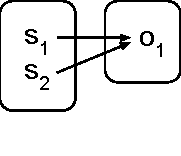
\includegraphics[width=.6\linewidth]{figures/state-aliasing}
  \caption{State Aliasing}
  \label{fig:state-aliasing}
\end{subfigure}
\begin{subfigure}{.3\textwidth}
  \centering
  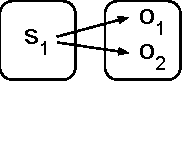
\includegraphics[width=.6\linewidth]{figures/noisy-perception}
  \caption{Noisy Perceptions}
  \label{fig:noisy-perception}
\end{subfigure}
\caption{A fully observed environment features a bijection between
  true states and observations. Partial observability indicates the
  degree to which this bijection is invalid. Two sources of partial
  observability are state aliasing, the degree to which the
  observation function is non-injective, and noisy perceptions, the
  degree to which the observation function is not a valid function.}
\label{fig:functions}
\end{figure}

\section{Sub-optimality induced by partial observability}
Partial observability causes agents to learn sub-optimal policies. The
degree of partial observability inherent in an environment bounds the
performance of an optimal policy learned over observations $\pi_O^*$
compared to the optimal policy learned over true states $\pi_S^*$:
\[
\textrm{sub-optimality} \propto \sum_{s\in S} D_{KL}\big(\pi_O^*(O(s))\ ||\ \pi_S^*(s)\big)
\]

\end{document}
